\qrchapter{https://forgottenpillar.com/rsc/en-fp-chapter11}{The personality of God - by James S. White}


\qrchapter{https://forgottenpillar.com/rsc/en-fp-chapter11}{Umbile la Mungu - na James S. White}


In what follows, we will examine James White’s pamphlet titled “\textit{The Personality of God}”. When we read this article, we will see that James White continues where Brother Loughborough left off, and that he expands and deepens the understanding behind the first point of the \emcap{Fundamental Principles}.


Katika kile kinachofuata, tutachunguza kijitabu cha James White chenye kichwa “\textit{Umbile la Mungu}”. Tunaposoma makala hii, tutaona kwamba James White anaendelea pale ambapo Ndugu Loughborough aliachia, na kwamba anapanua na kuongeza uelewa kwa hoja ya kwanza ya \emcap{Kanuni za Msingi}.


James White’s tract was printed multiple times, advertised 54 times, and reprinted twice in the Review and Herald publication. His view on the \emcap{personality of God} was well known and spread throughout Adventism. In this pamphlet, we will see clear criticism toward the ideas that Kellogg advocated in the Living Temple.


Trakti ya James White ilichapishwa mara nyingi, ikatangazwa mara 54, na kuchapishwa tena mara mbili ndani uchapishaji wa Review and Herald. Mtazamo wake juu ya \emcap{Umbile la Mungu} ulijulikana sana na kuenea katika Uadventista. Katika kijitabu hiki, tutaona ukosoaji wa wazi kuelekea mawazo ambayo Kellogg alitetea katika The Living Temple.


\begin{figure}[hp]
    \centering
    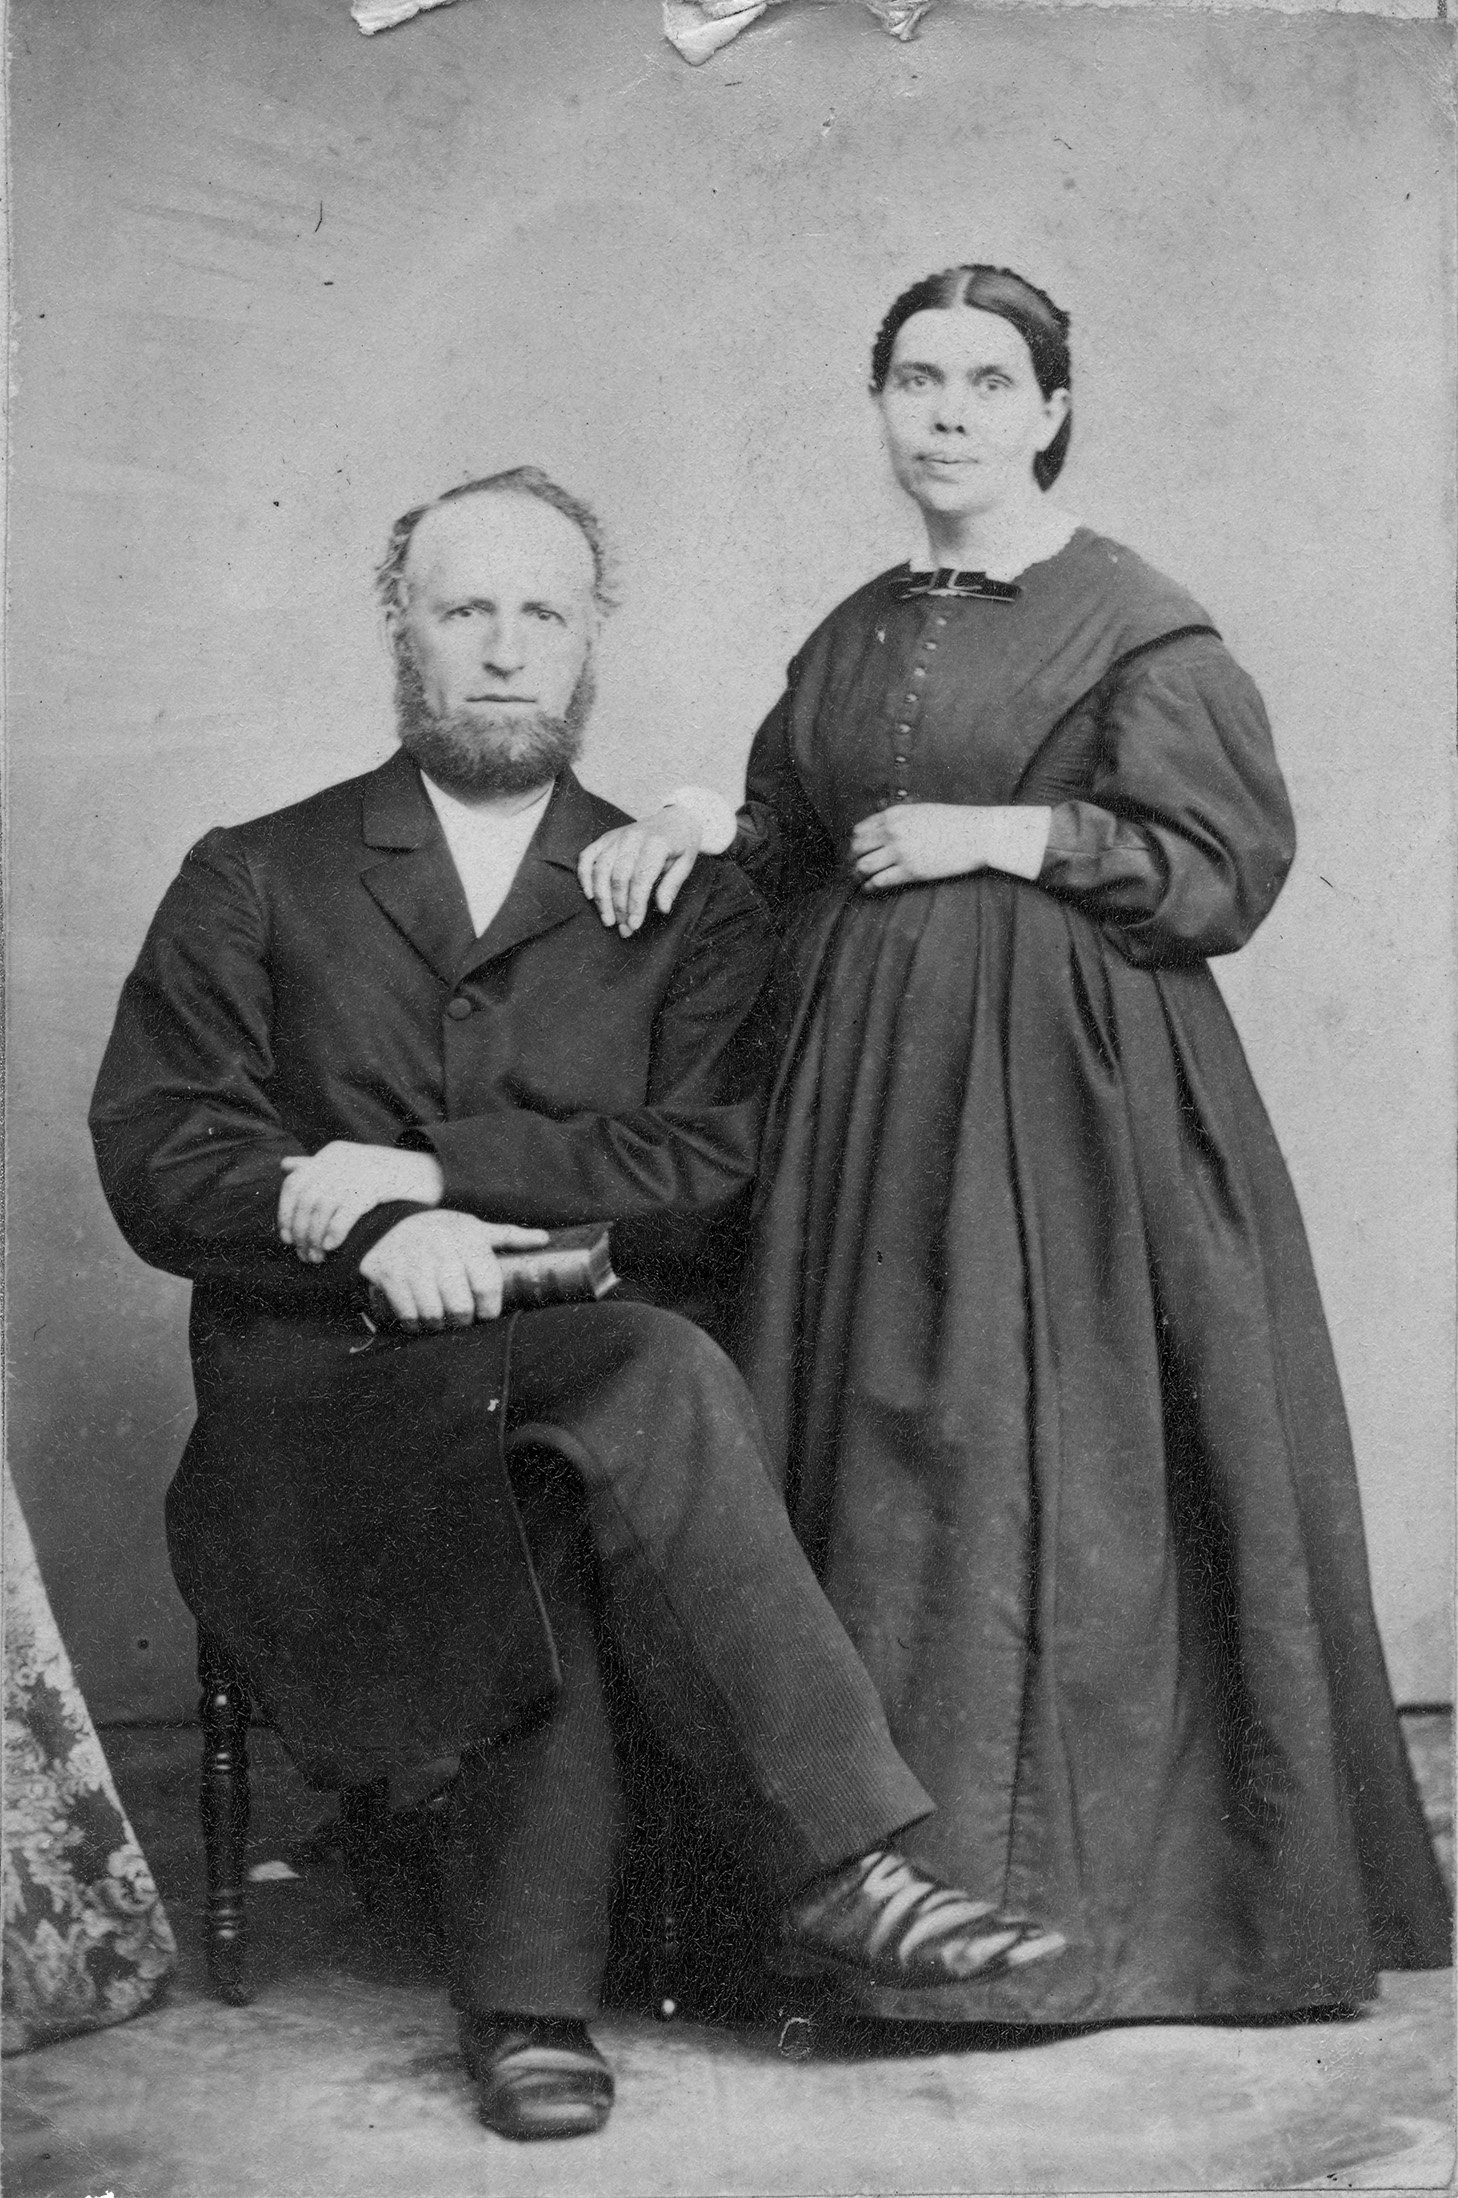
\includegraphics[width=1\linewidth]{images/james-and-ellen-white.jpg}
    \caption*{James Springer White (1821-1881) and Ellen White (1827-1915)}
    \label{fig:james-and-ellen-white}
\end{figure}


\begin{figure}[hp]
    \centering
    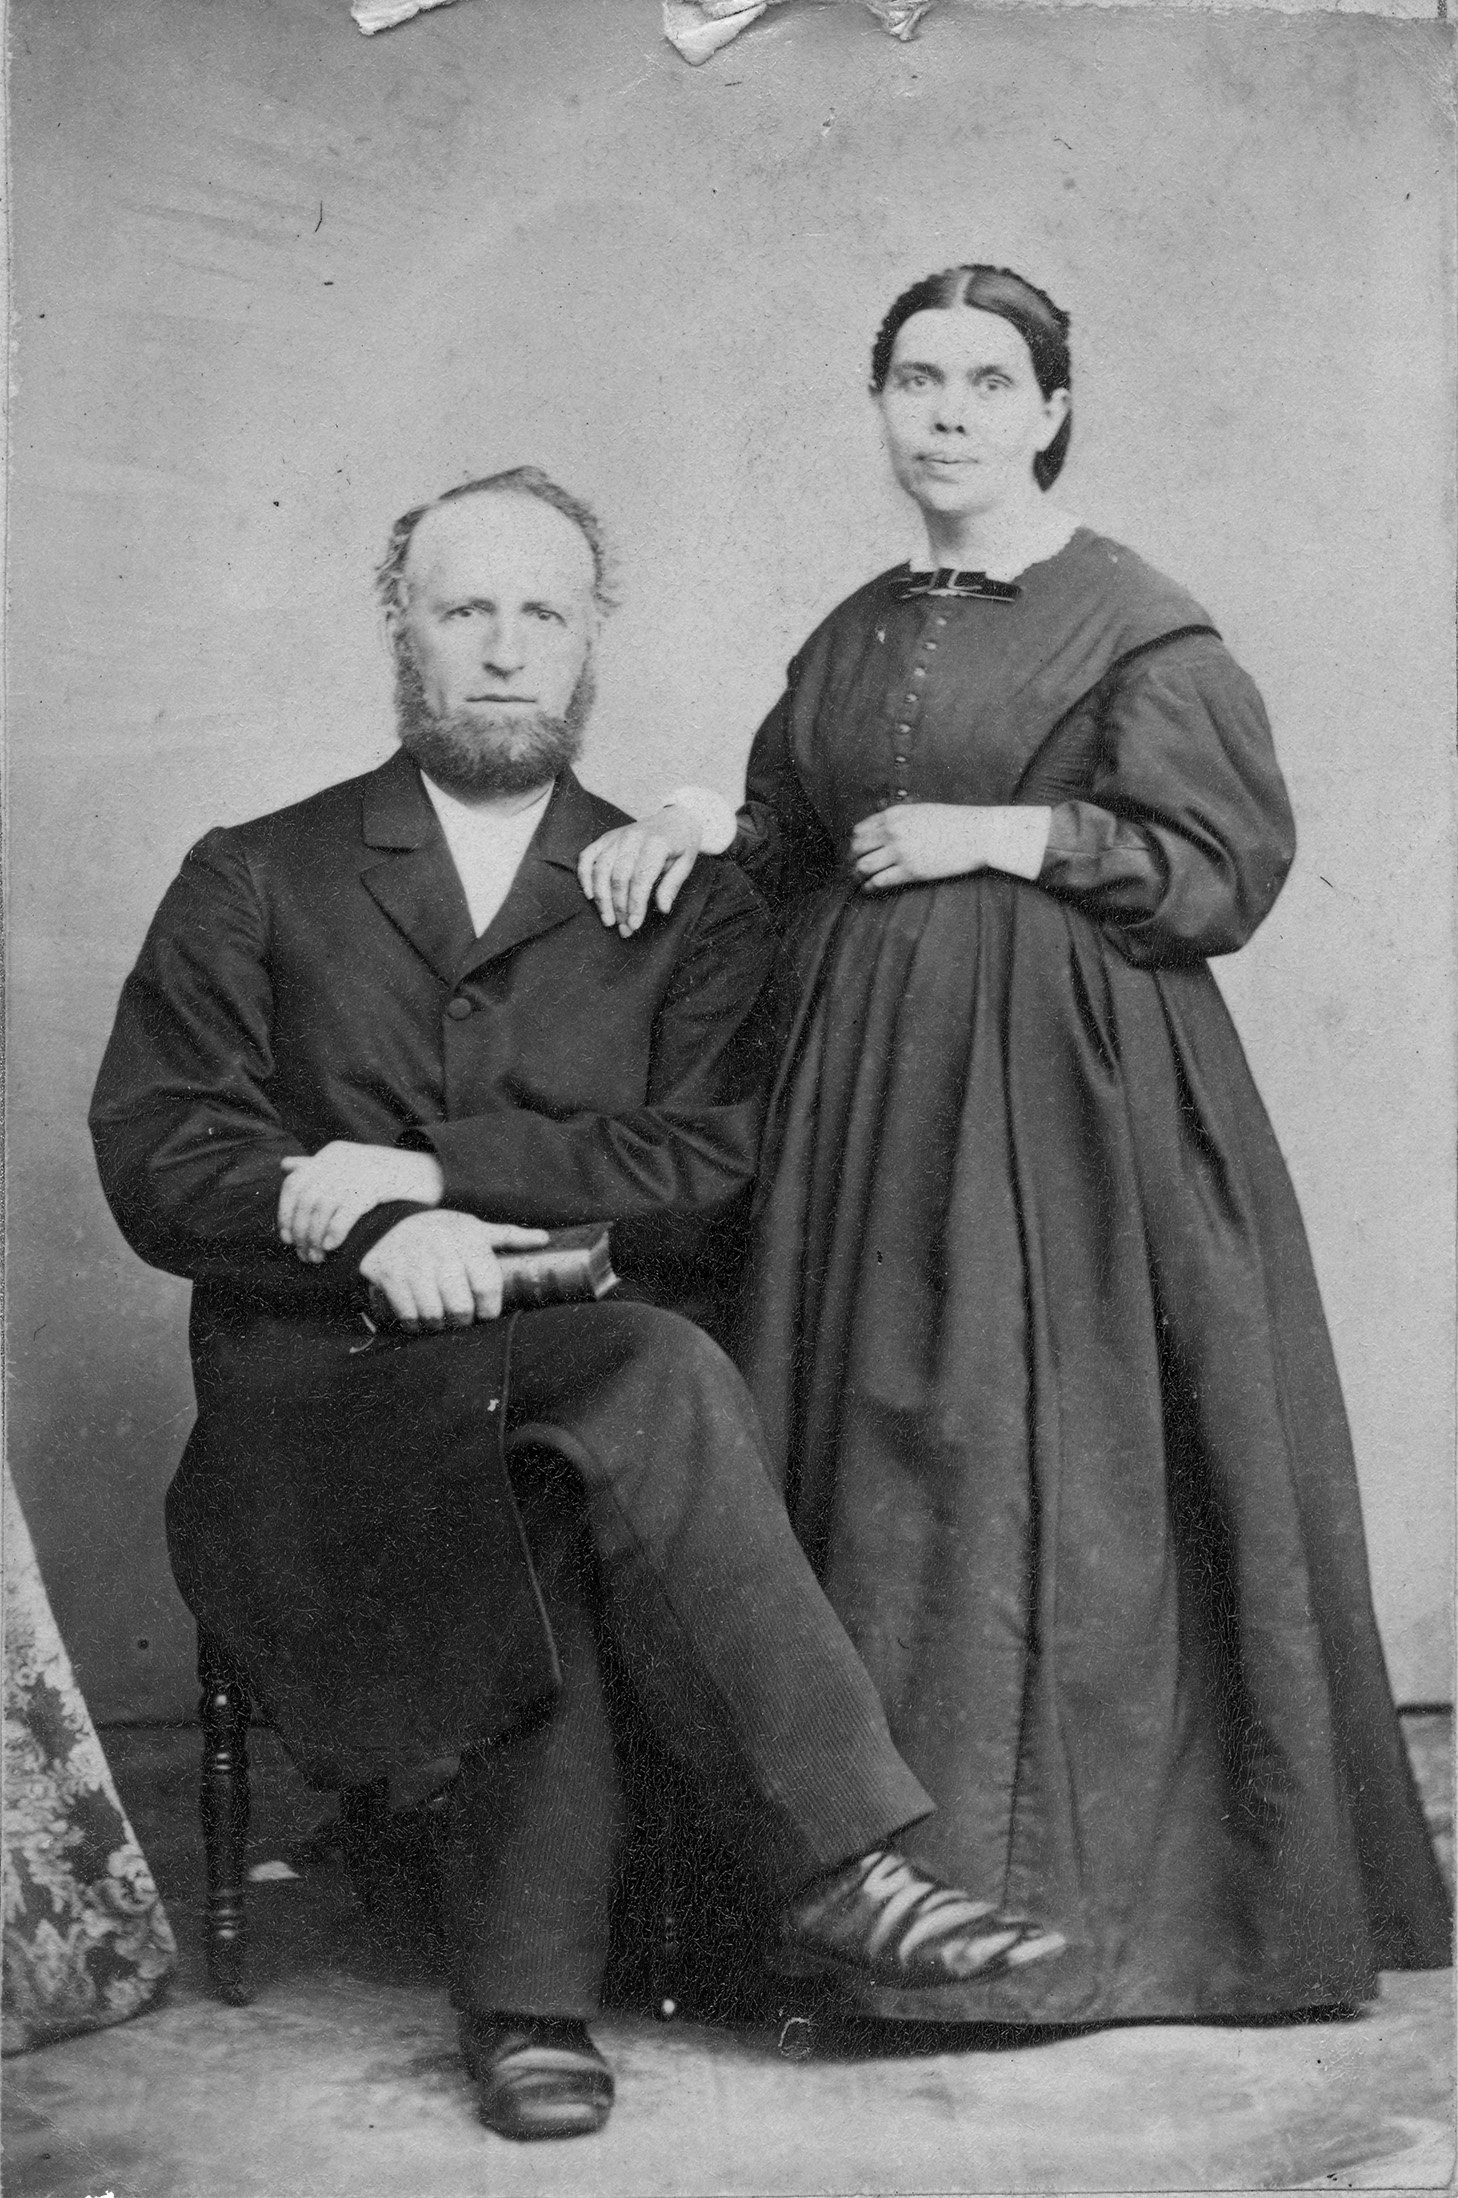
\includegraphics[width=1\linewidth]{images/james-and-ellen-white.jpg}
    \caption*{James Springer White (1821-1881) na Ellen White (1827-1915)}
    \label{fig:james-and-ellen-white}
\end{figure}


\othersQuote{\textbf{MAN was made in the image of God}. ‘And God said, Let us make man in our image, after our likeness.’ ‘So God created man in his own image, in the image of God created he him.’ Genesis 1:26, 27. See also chap. 9:6; 1 Corinthians 11:7. \textbf{Those who deny the personality of God, say that ‘image’ here does not mean \underline{physical form}, but moral image, and they make this the grand starting point to prove the immortality of all men}. The argument stands thus: First, man was made in God’s moral image. Second, God is an immortal being. Third, therefore all men are immortal. But this mode of reasoning would also prove man omnipotent, omniscient, and omnipresent, and thus clothe mortal man with all the attributes of the deity. Let us try it: First, man was made in God’s moral image. Second, God is omnipotent, omniscient, and omnipresent. Third, therefore, man is omnipotent, omniscient, and omnipresent. That which proves too much, proves nothing to the point, therefore the position that the image of God means his moral image, cannot be sustained. \textbf{As proof that God is a person, read his own words to Moses}: ‘And the Lord said, Behold there is a place by me, and thou shalt stand upon a rock; and it shall come to pass, while my glory passeth by, that I will put thee in a cleft of the rock, and will cover thee \textbf{with my hand} while \textbf{I pass by}. And I will take away \textbf{mine hand} and thou shalt \textbf{see my back parts}; \textbf{but my face shall not be seen}.’ Exodus 33:21-23. See also chap. 24:9-11. \textbf{Here God tells Moses that he shall \underline{see his form}}. \textbf{To say that God made it appear to Moses that he saw his form, when he has no form, is charging God with adding to falsehood a sort of juggling deception upon his servant Moses}.}[James S. White, PERGO 1.1; 1861][https://egwwritings.org/read?panels=p1471.3]


\othersQuote{\textbf{MWANADAMU aliumbwa kwa mfano wa Mungu}. ‘Mungu akasema, Na tumfanye mwanadamu kwa mfano wetu, baada ya namna yetu.’ ‘Basi Mungu akaumba mwanadamu kwa mfano wake, kwa mfano wa Mungu alimwumba.’ Mwanzo 1:26, 27. Ona pia sura ya. 9:6; 1 Wakorintho 11:7. \textbf{Wale wanaokataa Umbile la Mungu, wanasema kwamba ‘mfano’ hapa haimaanishi \underline{umbo la kimwili}, bali taswira ya kiadili, na wao hufanya hii iwe sehemu kuu ya kuanzia kuthibitisha kutokufa kwa watu wote}. Hoja inasimama hivi: Kwanza, mwanadamu aliumbwa kwa mfano wa Mungu wa kiadili. Pili, Mungu ni nafsi asiyeweza kufa. Tatu, kwa hiyo watu wote hawawezi kufa. Lakini namna hii ya kufikiri pia ingemthibitisha mwanadamu muweza wa yote, mjuzi wa yote, na aliye kila mahali, na hivyo kumvisha mwanadamu mwenye kufa sifa zote za mungu. Acheni tujaribu: Kwanza, mwanadamu aliumbwa kwa mfano wa Mungu wa kiadili. Pili, ni Mungu muweza wa yote, mjuzi wa yote, na aliye kila mahali. Tatu, kwa hivyo, mwanadamu ni muweza wa yote, mjuzi wa yote, na kila mahali. Kile ambacho kinathibitisha kupita kiasi, hakithibitishi chochote kwa uhakika, kwa hivyo msimamo kwamba mfano wa Mungu unamaanisha mfano wake wa maadili, hauwezi kudumu. \textbf{Kama ushahidi kwamba Mungu ni nafsi, soma maneno yake mwenyewe kwa Musa}: ‘Bwana akasema, Tazama, kuna mahali karibu nami, nawe utasimama juu ya mwamba; na itakuwa, wakati utukufu wangu ukipita, nitakuweka katika ufa wa mwamba, na kukufunika \textbf{kwa mkono wangu} \textbf{nikipita}. Nami nitauondoa \textbf{mkono wangu} nawe utaona \textbf{sehemu zangu za nyuma}; \textbf{lakini uso wangu haitaonekana}.’ Kutoka 33:21-23. Tazama pia sura. 24:9-11. \textbf{Hapa Mungu anamwambia Musa kwamba ataona \underline{umbo lake}}. \textbf{Kusema kwamba Mungu alimdhihirisha Musa kwamba aliona umbo lake, wakati yeye hana umbo, inamsingizia Mungu kwa kuongeza kwenye uwongo aina fulani ya mauzauza ya udanganyifu juu ya Musa mtumishi wake}.}[James S. White, PERGO 1.1; 1861][https://egwwritings.org/read?panels=p1471.3]


\othersQuoteNoGap{But the skeptic thinks he sees a contradiction between verse 11, which says that the Lord spake unto Moses face to face, and verse 20, which states that Moses could not see his face. But let Numbers 12:5-8 remove the difficulty. \textbf{‘And the Lord came down in the pillar of the cloud}, and stood in the door of the tabernacle, and called Aaron and Miriam, and they both came forth. And he said, Hear now my words. If there be a prophet among you, I, the Lord, will make myself known unto him in a vision, and will speak unto him in a dream. My servant Moses is not so, who is faithful in all mine house. \textbf{With him will I speak mouth to mouth, even \underline{apparently}}.’}[James S. White, PERGO 2.1; 1861][https://egwwritings.org/read?panels=p1471.6]


\othersQuoteNoGap{Lakini mwenye shaka anadhani anaona mgongano kati ya mstari wa 11, unaosema kwamba Bwana alizungumza na Musa uso kwa uso, na mstari wa 20, ambao unasema kwamba Musa hakuweza kuona uso wake. Wacha Hesabu 12:5-8 iondoe ugumu huo. \textbf{‘Na Bwana akashuka katika nguzo ya lile wingu}, akasimama mlangoni pa hema, akawaita Haruni na Miriamu, nao wote wawili wakatoka. Akasema, Sikieni sasa maneno yangu. Ikiwa kuna nabii kati yenu, mimi Bwana, nitajidhihirisha kwake katika maono, nami nitasema naye katika ndoto. Mtumishi wangu Musa si hivyo, ambaye ni mwaminifu katika nyumba yangu yote. \textbf{Pamoja naye nitazungumza mdomo kwa mdomo, hata \underline{kwa njia iliyo ya waziwazi}}.’}[James S. White, PERGO 2.1; 1861][https://egwwritings.org/read?panels=p1471.6]


\othersQuoteNoGap{The great and dreadful God came down, wrapped in a cloud of glory. \textbf{This cloud could be seen, but not the face which possesses more dazzling brightness than a thousand suns}. Under these circumstances Moses was permitted to draw near and \textbf{converse with God face to face, or mouth to mouth, even \underline{apparently}}.}[James S. White, PERGO 2.2; 1861][https://egwwritings.org/read?panels=p1471.7]


\othersQuoteNoGap{Mungu mkuu na wa kutisha alishuka, akiwa amevikwa wingu la utukufu. \textbf{Wingu hili liliweza kuonekana, lakini si uso ambao una mng'ao zaidi kuliko elfu jua}. Chini ya hali hizi Musa aliruhusiwa kukaribia na \textbf{kuzungumza na Mungu uso kwa uso, au mdomo kwa mdomo, hata kwa njia iliyo ya waziwazi}.}[James S. White, PERGO 2.2; 1861][https://egwwritings.org/read?panels=p1471.7]


\othersQuoteNoGap{Says the prophet Daniel, ‘I beheld till the thrones were cast down, and \textbf{the Ancient of days did sit}, whose garment was white as snow, \textbf{and the hairs of his head like the pure wool}; \textbf{his throne was like the fiery flame, and his wheels as burning fire}.’ Chap. 7:9. ‘I saw in the night visions, and, behold, one like the Son of man came with the clouds of heaven, and \textbf{came to the Ancient of days}, and they brought \textbf{him near before him}, and there was given him dominion and glory and a kingdom.’ Verses 13, 14.}[James S. White, PERGO 2.3; 1861][https://egwwritings.org/read?panels=p1471.8]


\othersQuoteNoGap{Nabii Danieli asema hivi, ‘Nikatazama hadi viti vya enzi vikashushwa, na \textbf{huyo mzee wa siku alikuwa ameketi}, ambaye vazi lake lilikuwa jeupe kama theluji, \textbf{na nywele za kichwa chake kama sufu safi}; \textbf{kiti chake cha enzi kilikuwa kama mwali wa moto, na magurudumu yake kama moto uwakao}.’ Sura 7:9. ‘Niliona katika maono ya usiku, na tazama, mmoja aliye kama Mwana wa Adamu akaja pamoja na mawingu ya mbinguni, na \textbf{akafika kwa huyo mzee wa siku}, wakamleta \textbf{karibu naye}, na pale akapewa uweza na utukufu na ufalme.’ Mistari ya 13, 14.}[James S. White, PERGO 2.3; 1861][https://egwwritings.org/read?panels=p1471.8]


\othersQuoteNoGap{Here is a sublime description of the action of \textbf{two personages}; viz, \textbf{God the Father, and his Son Jesus Christ}. \textbf{Deny their personality, and there is not a distinct idea in these quotations from Daniel}. In connection with this quotation read the apostle’s declaration that \textbf{the Son was in the express image of his Father’s person}. ‘God, who at sundry times, and in divers manners, spake in time past unto the fathers by the prophets, hath in these last days spoken unto us by his Son, whom he hath appointed heir of all things, by whom also he made the worlds; \textbf{who being the brightness of his glory, and the express image of his person}.’ Hebrews 1:1-3.}[James S. White, PERGO 3.1; 1861][https://egwwritings.org/read?panels=p1471.11]


\othersQuoteNoGap{Hapa kuna maelezo matukufu ya matendo ya \textbf{nafsi mbili}; yaani, \textbf{Mungu Baba, na Mwana wake Yesu Kristo}. \textbf{Kataa Umbile wao, na hakuna wazo tofauti katika nukuu hizi kutoka kwa Danieli}. Pamoja na nukuu hii soma tamko la mtume kwamba \textbf{Mwana alikuwa katika chapa dhahiri ya Umbile Wake}. ‘Mungu, ambaye nyakati za kale, na kwa njia nyingi alinena na baba zetu katika manabii, katika siku hizi za mwisho anasema nasi kupitia kwa Mwana, aliyemweka kuwa mrithi wa yote, tena kwa yeye aliumba ulimwengu; \textbf{ambaye ni mng'ao wa utukufu wake, na chapa dhahiri ya Umbile Wake}.’ Waebrania 1:1-3.}[James S. White, PERGO 3.1; 1861][https://egwwritings.org/read?panels=p1471.11]


\othersQuoteNoGap{We here add the testimony of Christ. ‘And the Father himself which hath sent me, hath borne witness of me. Ye have neither heard his voice at any time, \textbf{nor seen his shape}.’ John 5:37. See also Philippians 2:6. \textbf{To say that the Father has not a personal shape, seems the most pointed contradiction of plain scripture terms}. \\
OBJECTION. - ‘\textbf{\underline{God is a Spirit}}.’ John 4:24.}[James S. White, PERGO 3.2; 1861][https://egwwritings.org/read?panels=p1471.12]


\othersQuoteNoGap{Sisi hapa tunaongeza ushuhuda wa Kristo. ‘Na Baba mwenyewe aliyenituma alinishuhudia. Sauti yake hamjaisikia wakati wowote, \textbf{wala sura yake hamjaiona}.’ Yohana 5:37. Tazama pia Wafilipi 2:6. \textbf{Kusema kwamba Baba hana umbo la kibinafsi, inaonekana mkanganyiko ulio wazi zaidi wa maneno yaliyo wazi ya maandiko}. \\
PINGAMIZI. - ‘\textbf{\underline{Mungu ni Roho}}.’ Yohana 4:24.}[James S. White, PERGO 3.2; 1861][https://egwwritings.org/read?panels=p1471.12]


\othersQuoteNoGap{ANSWER. - \textbf{Angels are also spirits} [Psalm 104:4], yet those that visited Abram and Lot, lay down, ate, and took hold of Lot’s hand. \textbf{They were spirit beings. So is God a Spirit being}.}[James S. White, PERGO 3.3; 1861][https://egwwritings.org/read?panels=p1471.13]


\othersQuoteNoGap{JIBU. - \textbf{Malaika pia ni roho} [Zaburi 104:4], lakini wale waliowatembelea Abramu na Lutu, Wakalala, wakala, wakaushika mkono wa Lutu. Walikuwa viumbe wa kiroho. \textbf{Vivyo hivyo Mungu ni Huluki wa kiroho}.}[James S. White, PERGO 3.3; 1861][https://egwwritings.org/read?panels=p1471.13]


\othersQuoteNoGap{OBJ. - \textbf{God is everywhere}. Proof. Psalm 139:1-8. \textbf{He is as much in every place as in any one place}.}[James S. White, PERGO 3.4; 1861][https://egwwritings.org/read?panels=p1471.14]


\othersQuoteNoGap{OBJ. - \textbf{Mungu yuko kila mahali}. Ushahidi. Zaburi 139:1-8. \textbf{Yeye yuko zaidi katika kila mahali kama ilivyo katika sehemu nyingine}.}[James S. White, PERGO 3.4; 1861][https://egwwritings.org/read?panels=p1471.14]


\othersQuoteNoGap{ANS. - 1. \textbf{God is everywhere by virtue of his omniscience}, as will be seen by the very words of David referred to above. Verses 1-6. ‘O Lord, \textbf{thou hast searched me, and known me}. \textbf{Thou knowest} my down-sitting and mine uprising; \textbf{thou understandest} my thought afar off. Thou compassest my path and my lying down, and art \textbf{acquainted }with all my ways. For there is not a word in my tongue, but, lo, O Lord, \textbf{thou knowest it altogether}. Thou hast beset me behind and before, and laid thy hand upon me. \textbf{Such knowledge} is too wonderful for me. It is high; I cannot attain unto it.’}[James S. White, PERGO 3.5; 1861][https://egwwritings.org/read?panels=p1471.15]


\othersQuoteNoGap{ANS. - 1. \textbf{Mungu yuko kila mahali kwa uwezo wa kujua kwake yote}, kama itakavyoonekana kwa maneno ya Daudi yaliyotajwa hapo juu. Mistari ya 1-6. ‘Ee Bwana, \textbf{umenichunguza, na kunijua mimi}. \textbf{Wewe wajua} kuketi kwangu na kuinuka kwangu; \textbf{unaelewa} mawazo yangu kwa mbali. Umeizunguka njia yangu na kulala kwangu, na \textbf{unazifahamu} njia zangu zote. Kwa maana hamna neno katika ulimi wangu, lakini, tazama, Ee Bwana, \textbf{wewe wajua kabisa}. Wewe umenizingira nyuma na mbele, ukaweka mkono wako juu yangu. \textbf{Ujuzi kama huo} ni wa ajabu sana kwangu. Uko juu; Siwezi kuufikia.’}[James S. White, PERGO 3.5; 1861][https://egwwritings.org/read?panels=p1471.15]


\othersQuoteNoGap{2. \textbf{God is \underline{everywhere by virtue of his Spirit}, \underline{which is his representative}, and is manifested wherever he pleases}, as will be seen by the very words the objector claims, referred to above. Verses 7-10. ‘\textbf{Whither shall I go from \underline{thy Spirit}}? \textbf{or whither shall I flee from \underline{thy presence}}? If I ascend up into heaven, thou art there; if I make my bed in hell, behold, thou art there. If I take the wings of the morning, and dwell in the uttermost parts of the sea, even there shall thy hand lead me, and thy right hand shall hold me.’}[James S. White, PERGO 4.1; 1861][https://egwwritings.org/read?panels=p1471.18]


\othersQuoteNoGap{2. \textbf{Mungu yuko \underline{kila mahali kwa uwezo wa Roho wake}, \underline{ambaye ni mwakilishi wake}, na anadihirika popote apendapo}, kama itakavyoonekana kwa maneno ambayo mpingaji anadai, iliyotajwa hapo juu. Mistari wa 7-10. ‘\textbf{Nenda wapi niiache \underline{Roho yako}}? \textbf{au nitakimbilia wapi kutoka kwa \underline{uwepo wako}}? Nikipanda mbinguni, wewe uko huko; nikitandika kitanda changu kuzimu, tazama, uko huko. Nikichukua mbawa za asubuhi, na kukaa pande za mwisho za bahari, hata huko mkono wako utaniongoza, na mkono wako wa kuume utanishika.’}[James S. White, PERGO 4.1; 1861][https://egwwritings.org/read?panels=p1471.18]


\othersQuoteNoGap{\textbf{God is in heaven.} This we are taught in the Lord’s prayer. ‘\textbf{Our Father which art in heaven}.’ Matthew 6:9; Luke 11:2. \textbf{But if God is as much in every place as he is in any one place, then heaven is also as much in every place as it is in any one place, and the idea of going to heaven is all a mistake}. We are all in heaven; and the Lord’s prayer, according to this foggy theology simply means, Our Father \textbf{which art everywhere,} hallowed be thy name. Thy kingdom come, thy will be done, on earth, \textbf{as it is everywhere}.}[James S. White, PERGO 4.2; 1861][https://egwwritings.org/read?panels=p1471.19]


\othersQuoteNoGap{\textbf{Mungu yuko mbinguni}. Haya tunafundishwa katika maombi ya Bwana. ‘\textbf{Baba yetu uliye juu mbinguni}.’ Mathayo 6:9; Luka 11:2. \textbf{Lakini ikiwa Mungu yuko katika kila mahali kama alivyo mahali popote pamoja, basi mbingu pia iko katika kila mahali kama ilivyo mahali pamoja, na wazo la kwenda mbinguni yote ni makosa}. Sisi sote tuko mbinguni; na maombi ya Bwana, kulingana na teolojia hii ya ukungu ina maana kwa urahisi, Baba yetu \textbf{ambaye yuko kila mahali,} Jina lako litukuzwe. Ufalme wako na uje, mapenzi yako yatimizwe, duniani, \textbf{kama kila mahali}.}[James S. White, PERGO 4.2; 1861][https://egwwritings.org/read?panels=p1471.19]


\othersQuoteNoGap{Again, Bible readers have believed that Enoch and Elijah were really taken up \textbf{to God in heaven}. \textbf{But if God and heaven be as much in every place as in any one place, this is all a mistake}. They were not translated. And all that is said about the chariot of fire, and horses of fire, and the attending whirlwind to take Elijah up into heaven, was a useless parade. They only evaporated, and a misty vapor passed through the entire universe. This is all of Enoch and Elijah that the mind can possibly grasp, \textbf{admitting that God and heaven are no more in any one place than in every place}. But it is said of Elijah that he ‘\textbf{went up} by a whirlwind \textbf{into heaven}.’ 2 Kings 2:11. And of Enoch it is said that he ‘walked with God, and was not, for God took him.’ Genesis 5:24.}[James S. White, PERGO 4.3; 1861][https://egwwritings.org/read?panels=p1471.20]


\othersQuoteNoGap{Tena, wasomaji wa Biblia wameamini kwamba Enoko na Eliya kwa kweli walichukuliwa \textbf{hadi kwa Mungu mbinguni}. \textbf{Lakini ikiwa Mungu na mbingu ziko kila mahali kama ilivyo mahali pamoja, haya yote ni makosa}. Hawakutafsiriwa. Na yote yanayosemwa kuhusu gari la moto, na farasi wa moto, na upepo wa kisulisuli wa kumchukua Eliya juu mbinguni, ilikwa tu gwaride ya upuzi. Walivukiza tu, na mvuke wa ukungu ukapita ulimwengu mzima. Hii ni yote kuhusu Enoko na Eliya ambayo akili inaweza kufahamu, \textbf{ikikubalika kwamba Mungu na mbingu wako katika sehemu moja kuliko kila mahali}. Lakini inasemwa juu ya Eliya kwamba ‘\textbf{alipanda} kwa kisulisuli \textbf{mbinguni}.’ 2 Wafalme 2:11. Na kuhusu Henoko inasemekana kwamba ‘alitembea pamoja na Mungu, naye hayuko, kwa kuwa Mungu alimchukua.’ Mwanzo 5:24.}[James S. White, PERGO 4.3; 1861][https://egwwritings.org/read?panels=p1471.20]


\othersQuoteNoGap{\textbf{Jesus is said to be on the right hand of the Majesty on high}. Hebrews 1:3. ‘So, then, after the Lord had spoken unto them \textbf{he was received \underline{up into heaven}}, \textbf{and sat on the right hand of God}.’ Mark 16:19. \textbf{But if heaven be everywhere, and God everywhere, then Christ’s ascension up to heaven, at the Father’s right hand, simply means that he went everywhere}! He was only taken up where the cloud hid him from the gaze of his disciples, and then evaporated and went everywhere! So that instead of the lovely Jesus, so beautifully described in both Testaments, we have only a sort of essence dispersed through the entire universe. And in harmony with this rarified theology, Christ’s second advent, or his return, would be the condensation of this essence to some locality, say the mount of Olivet! \textbf{Christ arose from the dead with a physical form}. ‘He is not here,’ said the angel, ‘for he is risen as he said.’ Matthew 28:6.}[James S. White, PERGO 5.1; 1861][https://egwwritings.org/read?panels=p1471.23]


\othersQuoteNoGap{\textbf{Inasemekana Yesu yuko mkono wa kuume wa Ukuu huko juu}. Waebrania 1:3. ‘Basi, baada ya Bwana kusema nao \textbf{alichukuliwa \underline{juu mbinguni}}, \textbf{akaketi juu yake mkono wa kuume wa Mungu}.’ Marko 16:19. \textbf{Lakini ikiwa mbingu yuko kila mahali, na Mungu kila mahali, kisha kupaa kwa Kristo mbinguni, kwenye mkono wa kuume wa Baba, kunamaanisha tu kwamba yeye alienda kila mahali}! Alichukuliwa tu juu ambapo wingu lilimficha kutoka kwa macho ya wanafunzi wake, na kisha kuyeyuka na kwenda kila mahali! Ili kwamba badala ya Yesu mpendwa, iwe hivyo ilivyoelezwa kwa uzuri katika Agano zote mbili, tuna aina fulani tu ya kiini kilichotawanywa ulimwengu mzima. Na kupatana na theolojia hii iliyothibitishwa, ujio wa pili wa Kristo, au kurudi kwake itakuwa ni ufupisho wa kiini hiki kwa eneo fulani, sema mlima wa Mizeituni! \textbf{Kristo alifufuka kutoka kwa wafu akiwa na umbo la kimwili}. ‘Hayupo hapa,’ akasema malaika, ‘kwa maana yuko kufufuka kama alivyosema.’ Mathayo 28:6.}[James S. White, PERGO 5.1; 1861][https://egwwritings.org/read?panels=p1471.23]


\othersQuoteNoGap{‘And as they went to tell his disciples, behold, Jesus met them, saying, All hail! And they came and \textbf{held him by the feet}, and they worshiped him.’ Verse 9.}[James S. White, PERGO 5.2; 1861][https://egwwritings.org/read?panels=p1471.24]


\othersQuoteNoGap{‘Na walipokuwa wakienda kuwaambia wanafunzi wa Yesu tazama, Yesu akakutana nao, akiwasalimu, Salamu! Na wao wakaja \textbf{wakamshika miguu}, wakamsujudia.’ Mstari wa 9.}[James S. White, PERGO 5.2; 1861][https://egwwritings.org/read?panels=p1471.24]


\othersQuoteNoGap{‘\textbf{Behold my hands and my feet},’ said Jesus to those who stood in doubt of his resurrection, ‘that it is I myself. \textbf{Handle me and see, \underline{for a spirit hath not flesh and bones} as ye see me have}. And when he had thus spoken, he \textbf{showed them his hands and his feet}. And while they yet believed not for joy, and wondered, he said unto them, Have ye here any meat? And they gave him a piece of broiled fish, and of an honey-comb, and he took it and did eat before them.’ Luke 24:39-43.}[James S. White, PERGO 5.3; 1861][https://egwwritings.org/read?panels=p1471.25]


\othersQuoteNoGap{‘\textbf{Tazama mikono yangu na miguu yangu},’ Yesu akawaambia wale waliokuwa na shaka naye ufufuo, ‘kwamba ni mimi mwenyewe. \textbf{Nishikeni mwone, \underline{maana roho haina nyama na mifupa} kama mnavyoniona ninavyo}. Naye akiisha kusema hayo, \textbf{akawaonyesha mikono yake na miguu yake}. Na walipokuwa bado hawajaamini kwa furaha, wakistaajabu, akawaambia, Je! mna nyama yoyote? Wakampa kipande cha samaki wa kuokwa, na sega la asali, akakitwaa na kula mbele yao.’ Luka 24:39-43.}[James S. White, PERGO 5.3; 1861][https://egwwritings.org/read?panels=p1471.25]


\othersQuoteNoGap{After Jesus addressed his disciples on the mount of Olivet, he \textbf{was taken up from them}, and a cloud received him out of their sight. ‘And while they looked steadfastly \textbf{toward heaven as he went up,} behold two men stood by them in white apparel, which also said, Ye men of Galilee, why stand ye gazing up into heaven? This same Jesus which is \textbf{taken up from you into heaven}, shall so come in like manner as ye have seen him \textbf{go into heaven}.’ Acts 1:9-11. J. W.}[James S. White, PERGO 6.1; 1861][https://egwwritings.org/read?panels=p1471.27]


\othersQuoteNoGap{Baada ya Yesu kusema na wanafunzi wake katika mlima wa Mizeituni, \textbf{alipandishwa kutoka kwao}, na wingu likampokea kutoka machoni pao. ‘Na huku wakitazama kwa uthabiti \textbf{alipokuwa akienda mbinguni,} tazama, watu wawili wakasimama karibu nao, wenye mavazi meupe, wakasema, Ninyi Enyi watu wa Galilaya, mbona mmesimama mkitazama mbinguni? Yesu huyu huyu ambaye \textbf{amechukuliwa juu kutoka kwenu kwenda mbinguni}, atakuja jinsi iyo hiyo mlivyomwona \textbf{akienda zake mbinguni}.’ Matendo 1:9-11. J. W.}[James S. White, PERGO 6.1; 1861][https://egwwritings.org/read?panels=p1471.27]


James White fights the idea that God is just a spirit, and as such, is present \others{as much in every place as in any one place}. He gives plain and positive testimony from Scripture that God is a personal being; we see the very same sentiments in Ellen White’s writings.


James White anapinga wazo la kwamba Mungu ni roho tu, na kwa hivyo, yuko \others{zaidi katika kila mahali kama mahali pamoja}. Anatoa ushuhuda wa wazi na chanya kutoka katika Maandiko kwamba Mungu ni huluki binafsi; tunaona hisia sawa katika maandishi ya Ellen White.


\egw{The mighty power that works through all nature and sustains all things is not, as some men of science claim, \textbf{merely an all-pervading principle}, an actuating energy. \textbf{\underline{God is a spirit; yet He is a personal being}}, \textbf{for man was made in His image}. \textbf{As \underline{a personal being}}, God has revealed Himself in His Son. Jesus, the outshining of the Father’s glory, “and \textbf{the express \underline{image of His person}}” (Hebrews 1:3), was on earth found in fashion as a man. As \textbf{a personal Saviour} He came to the world. As \textbf{a personal Saviour He ascended \underline{on high}}. As \textbf{a personal Saviour He intercedes \underline{in the heavenly courts}}. \textbf{Before the throne of God} in our behalf ministers “One like the Son of man.” Daniel 7:13.}[Ed 131.5; 1903][https://egwwritings.org/read?panels=p29.632]


\egw{Nguvu kuu inayofanya kazi kupitia maumbile yote na kutegemeza vitu vyote si, kama watu wengine wanasayansi wanavyodai, \textbf{kanuni inayoenea tu}, nishati inayofanya kazi. \textbf{\underline{Mungu ni roho; lakini Yeye ni huluki binafsi}}, \textbf{kwa maana mwanadamu aliumbwa kwa mfano Wake}. \textbf{Kama \underline{mtu binafsi}}, Mungu amejidhihirisha katika Mwanawe. Yesu, mng'ao wa utukufu wa Baba, “na \textbf{mfano halisi \underline{wa nafsi yake}}” (Waebrania 1:3), alikuwa duniani alionekana katika umbo kama mwanadamu. Kama \textbf{Mwokozi binafsi} Alikuja ulimwenguni. Kama \textbf{Mwokozi binafsi alipaa \underline{juu}}. Kama \textbf{Mwokozi wa kibinafsi Yeye hufanya maombezi \underline{katika nyua za mbinguni}}. \textbf{Mbele ya kiti cha enzi cha Mungu} kwa niaba yetu wanahudumu “Mmoja kama Mwana wa binadamu.” Danieli 7:13.}[Ed 131.5; 1903][https://egwwritings.org/read?panels=p29.632]


Ellen White and the Adventist pioneers made a distinction between the terms ‘\textit{spirit}’ and ‘\textit{being}’. God is a personal being, not just a spirit. He is not\others{as much in every place as in any one place}, but He is\others{in one place more than another}[John. N. Loughborough, “Is God a Person?” The Adventist Review and Sabbath Herald, September 18, 1855][https://documents.adventistarchives.org/Periodicals/RH/RH18550918-V07-06.pdf]. He is in heaven, in His temple, sitting on His throne—in person—and He is everywhere present by His representative, the Holy Spirit.


Ellen White na waanzilishi wa Waadventista walifanya tofauti kati ya maneno ‘roho’ na ‘huluki’. Mungu ni huluki binafsi, si roho tu. Yeye hayuko\others{zaidi katika kila mahali kama mahali pamoja}, lakini Yeye yuko\others{mahali pamoja zaidi ya mahali pengine}[John. N. Loughborough, “Is God a Person?” The Adventist Review and Sabbath Herald, September 18, 1855][https://documents.adventistarchives.org/Periodicals/RH/RH18550918-V07-06.pdf]. Yuko mbinguni, katika hekalu lake, ameketi juu ya kiti Chake cha enzi—katika nafsi—na Yeye yuko kila mahali kupitia kwa mwakilishi Wake, Roho mtakatifu.


Here are some other quotations from Sister White that are in harmony with the pioneers’ views on the \emcap{personality of God}:


Hapa kuna manukuu mengine kutoka kwa Dada White ambayo yanapatana na waanzilishi katika maoni juu ya \emcap{ubinafsi wa Mungu}:


\egw{He \normaltext{[Jesus]} taught that God was a rewarder of the righteous, and a punisher of the transgressor. \textbf{He was not an intangible spirit}, but a living ruler of the universe. \textbf{This gracious Father} was constantly working for the good of man, and mindful of all that concerns him...}[3SP 47.1; 1878][https://egwwritings.org/read?panels=p142.195]


\egw{Yeye \normaltext{[Yesu]} alifundisha kwamba Mungu ni mthawabishaji wa wenye haki, na muadhibu wa wenye haki mvunja sheria. \textbf{Hakuwa roho isiyoshikika}, bali mtawala aliye hai wa ulimwengu. \textbf{Huyu Baba mwenye neema} alikuwa akifanya kazi kila mara kwa ajili ya wema wa mwanadamu, na kukumbuka yote hayo inamhusu...}[3SP 47.1; 1878][https://egwwritings.org/read?panels=p142.195]


\egw{\textbf{The Bible shows us \underline{God in His high and holy place}}, not in a state of inactivity, not in silence and solitude, but surrounded by ten thousand times ten thousand and thousands of thousands of holy beings, all waiting to do His will. \textbf{Through these messengers He is in active communication with every part of His dominion}. \textbf{\underline{By His Spirit He is everywhere present}}. \textbf{Through the agency of His Spirit and His angels} He ministers to the children of men.}[MH 417.2; 1905][https://egwwritings.org/read?panels=p135.2136]


\egw{\textbf{Biblia inatuonyesha \underline{Mungu katika mahali pake pa juu na patakatifu}}, si katika hali ya kutotenda, si katika ukimya na upweke, lakini amezungukwa na elfu kumi mara elfu kumi na maelfu ya maelfu ya viumbe watakatifu, wote wakingoja kufanya mapenzi Yake. \textbf{Kupitia wajumbe hawa Yeye yuko katika mawasiliano hai na kila sehemu ya utawala Wake}. \textbf{\underline{Kupitia kwa Roho wake yuko kila mahali sasa}}. \textbf{Kupitia wakala wa Roho wake na malaika zake} anawahudumia watoto wa wanaume.}[MH 417.2; 1905][https://egwwritings.org/read?panels=p135.2136]


\egw{The greatness of God is to us incomprehensible. ‘\textbf{The Lord’s throne is in heaven}’ (Psalm 11:4); \textbf{\underline{yet by His Spirit He is everywhere present}}. \textbf{He has an intimate knowledge} of, and a personal interest in, all the works of His hand.}[Ed 132.2; 1903][https://egwwritings.org/read?panels=p29.636]


\egw{Ukuu wa Mungu kwetu sisi haueleweki. ‘\textbf{Kiti cha enzi cha Bwana ki mbinguni}’ (Zaburi 11:4); \textbf{\underline{lakini kwa Roho wake yuko kila mahali}}. \textbf{Ana ujuzi wa ndani} wa, na shauku ya kibinafsi katika, kazi zote za mkono Wake.}[Ed 132.2; 1903][https://egwwritings.org/read?panels=p29.636]


\egw{Through Jesus Christ, \textbf{God—not a perfume, \underline{not something intangible}, \underline{but a personal God}}—created man and endowed him with intelligence and power.}[Ms117-1898.10; 1898][https://egwwritings.org/read?panels=p7182.15]


\egw{Kupitia Yesu Kristo, \textbf{Mungu—si manukato, \underline{si kitu kisichoshikika}, \underline{bali Mungu binafsi}}—aliyemuumba mwanadamu na kumpa akili na uwezo.}[Ms117-1898.10; 1898][https://egwwritings.org/read?panels=p7182.15]


Continuing in James White’s pamphlet, we read his sharp criticism on the notion of an immaterial God. Before that, let’s briefly recall Dr. Kellogg’s argument that\others{\textbf{\underline{Discussions respecting the form of God are utterly unprofitable}}}[Dr. John H. Kellogg, The Living Temple, p.33.][https://archive.org/details/J.H.Kellogg.TheLivingTemple1903/page/n33/] because God is\others{\textbf{far beyond our comprehension }\textbf{\underline{as are the bounds of space and time}}}. He believed that God’s person is not constrained to one locality because He is in\others{as much in every place as in any one place}[James S. White, PERGO 4.3; 1861][https://egwwritings.org/read?panels=p1471.20] \footnote{In the Living Temple, Dr. Kellogg objected that God cannot be everywhere presente at once: “\textit{Says one}, ‘God may be present by his Spirit, or by his power, but certainly God himself \textit{cannot be present everywhere at once}.’ We answer: How can power be separated from the source of power? Where God’s Spirit is at work, where God’s power is manifested, God \textit{himself is actually and truly present}…” \href{https://archive.org/details/J.H.Kellogg.TheLivingTemple1903/page/n29/}{John H. Kellogg, The Living Temple, p.28}.}. If God in His personality were truly a definite being, having a tangible body, then He would not be able to be present\others{as much in every place as in any one place} and, thus, sustain life. James White continues against the reasoning that God is immaterial in His person.


Tukiendelea katika kijitabu cha James White, tunasoma ukosoaji wake mkali juu ya dhana ya Mungu asiye na mwili. Kabla ya hapo, hebu tukumbuke kwa ufupi hoja ya Dk. Kellogg kwamba\others{\textbf{\underline{Majadiliano kuhusu umbo la Mungu hayana faida kabisa}}}[Dr. John H. Kellogg, The Living Temple, p.33.][https://archive.org/details/J.H.Kellogg.TheLivingTemple1903/page/n33/] kwa sababu Mungu \others{\textbf{yuko mbali sana na sisi \textbf{\underline{kwa ufahamu kama vile ilivyo mipaka ya nafasi na wakati}}}}. Aliamini kwamba nafsi ya Mungu ni hailazimiki katika eneo moja kwa sababu Yeye yuko\others{zaidi kila mahali kama mahali pamoja}[James S. White, PERGO 4.3; 1861][https://egwwritings.org/read?panels=p1471.20] \footnote{Katika Hekalu Hai, Dk. Kellogg alipinga kwamba Mungu hawezi kuwa kila mahali kwa wakati mmoja: “\textit{Asema mmoja}, ‘Mungu anaweza kuwepo kwa Roho wake, au kwa nguvu zake, lakini hakika Mungu mwenyewe \textit{hawezi kuwepo kila mahali kwa wakati mmoja}.’ Tunajibu: Nguvu zinawezaje kutenganishwa na chanzo cha nguvu? Mahali ambapo Roho wa Mungu anafanya kazi, mahali ambapo nguvu za Mungu zinadhihirishwa, Mungu \textit{mwenyewe kwa kweli na kwa hakika yupo}…“ \href{https://archive.org/details/J.H.Kellogg.TheLivingTemple1903/page/n29/}{John H. Kellogg, The Living Temple, p.28}.}. Ikiwa Mungu katika ubinafsi Wake angekuwa huluki dhahiri, mwenye mwili unaoshikika, basi hangeweza kuwepo\others{zaidi kila mahali kama mahali pamoja} na, hivyo, kudumisha maisha. James White anaendelea dhidi ya hoja kwamba Mungu hana mwili katika nafsi yake.


\othersQuote{IMMATERIALITY}


\othersQuote{KUTOKUWA NA MWILI}


\othersQuoteNoGap{\textbf{THIS is but another name for nonentity}. \textbf{It is the negative of all} \textbf{things and} \textbf{\underline{beings} }- of all existence. There is not one particle of proof to be advanced to establish its existence. It has no way to manifest itself to any intelligence in heaven or on earth. \textbf{Neither God, angels, nor men could possibly conceive of such a substance, being, or thing}. \textbf{It possesses no property or power by which \underline{to make itself manifest to any intelligent being} in the universe}. Reason and analogy never scan it, or even conceive of it. \textbf{Revelation never reveals it, nor do any of our senses witness its existence}. \textbf{It cannot be seen, felt, heard, tasted, or smelled, even by the strongest organs, or the most acute sensibilities}. It is neither liquid nor solid, soft nor hard - it can neither extend nor contract. In short, it can exert no influence whatever - it can neither act nor be acted upon. And even if it does exist, it can be of no possible use. It possesses no one, desirable property, faculty, or use, yet, strange to say, \textbf{immateriality is the modern Christian’s God}, \textbf{his anticipated heaven}, \textbf{his immortal self} - \textbf{his all}!}[James S. White, PERGO 6.2; 1861][https://egwwritings.org/read?panels=p1471.29]


\othersQuoteNoGap{\textbf{HILI ni jina lingine tu la chaupepeta}. \textbf{Ni hasi ya vitu} \textbf{vyote na} \textbf{\underline{huluki} }- ya vyote kuwepo. Hakuna chembe hata moja cha uthibitisho wa kuendelezwa ili kuthibitisha kuwepo kwake. Haina njia ya kujidhihirisha kwa akili yoyote mbinguni au nchini. \textbf{Mungu, malaika, na wanadamu hawawezi kufikiria kitu kama hicho, kiumbe au kitu kama hicho}. \textbf{Haimiliki mali au nguvu yoyote ambayo kwayo \underline{inaweza kujidhihirisha kwa kiumbe chochote chenye akili ulimwenguni}}. Wazo na mlinganisho kamwe hazichanganui, au hata kuzifikiria. \textbf{Ufunuo kamwe haufichui wala hakuna hisia zetu kushuhudia kuwepo kwake}. \textbf{Haiwezi kuonekana, kuhisika, kusikika, kuonjeka, au kunusika, hata kwa viungo vya nguvu zaidi, au hisia kali zaidi}. Sio kioevu au ngumu, laini au ngumu - haiwezi kupanua au kupungua. Kwa ufupi, haiwezi kuwa na ushawishi wowote - haiwezi kuchukua hatua au kutekelezwa. Na hata kama ipo, haiwezi kutumika. Haina mtu yeyote, mali inayohitajika, kitivo, au kazi, hata hivyo, ajabu kusema, \textbf{kutokuwa na mwili ni Mungu wa Mkristo wa kisasa}, \textbf{mbingu yake anayotarajia}, \textbf{nafsi yake isiyoweza kufa} - \textbf{yake yote}!}[James S. White, PERGO 6.2; 1861][https://egwwritings.org/read?panels=p1471.29]


\othersQuoteNoGap{\textbf{O sectarianism! O atheism!! O annihilation!!!} \textbf{who can perceive the nice shades of difference between the one and the other?} They seem alike, all but in name. \textbf{The atheist has no God. \underline{The sectarian has a God without body or parts}.} Who can define the difference? For our part we do not perceive a difference of a single hair; \textbf{they both claim to be the negative of all things which exist} - and both are equally powerless and unknown.}[James S. White, PERGO 6.3; 1861][https://egwwritings.org/read?panels=p1471.30]


\othersQuoteNoGap{\textbf{Enyi madhehebu! O Asiyeamini Mungu!! O maangamizi!!!} \textbf{nani anaweza kutambua vivuli vyema vya tofauti kati ya moja na nyingine?} Wanaonekana sawa, wote isipokuwa kwa jina. \textbf{Mkana Mungu hana Mungu. \underline{Mdhehebu ana Mungu asiye na mwili au sehemu}.} Nani anaweza kufafanua tofauti? Kwa upande wetu hatuoni tofauti ya unywele mmoja; \textbf{wote wawili wanadai kuwa hasi ya vitu vyote vilivyopo} - na vyote viwili havina nguvu na havijulikani.}[James S. White, PERGO 6.3; 1861][https://egwwritings.org/read?panels=p1471.30]


\othersQuoteNoGap{\textbf{The atheist has no after life, or conscious existence beyond the grave. The sectarian has one, \underline{but it is immaterial, like his God; and without body or parts}. Here again both are negative, and both arrive at the same point}. Their faith and hope amount to the same; only it is expressed by different terms.}[James S. White, PERGO 7.1; 1861][https://egwwritings.org/read?panels=p1471.33]


\othersQuoteNoGap{\textbf{Mtu asiyeamini kuwa kuna Mungu hana maisha ya baadaye, zaidi ya kaburi. Mdhehebu ana moja, \underline{lakini haionekani, kama Mungu wake; na bila mwili au sehemu}. Hapa tena wote wawili ni hasi, na wote wawili wanafika katika hatua moja}. Imani na tumaini lao ni sawa; ila inaonyeshwa kwa maneno tofauti.}[James S. White, PERGO 7.1; 1861][https://egwwritings.org/read?panels=p1471.33]


\othersQuoteNoGap{Again, \textbf{the atheist has no heaven in eternity}. \textbf{The sectarian has one, but it is \underline{immaterial in all its properties}, and is therefore the negative of all riches and substances}. Here again they are equal, and arrive at the same point.}[James S. White, PERGO 7.2; 1861][https://egwwritings.org/read?panels=p1471.34]


\othersQuoteNoGap{Tena, \textbf{asiyeamini Mungu hana mbingu katika umilele}. \textbf{Mdhehebu ana mmoja, lakini \underline{haionekani katika mali zake zote}, na kwa hiyo hasi katika mali na vitu vyote}. Hapa tena wako sawa, na wanafikia hatua sawa.}[James S. White, PERGO 7.2; 1861][https://egwwritings.org/read?panels=p1471.34]


\othersQuoteNoGap{As we do not envy them the possession of all they claim, we will now leave them in the quiet and undisturbed enjoyment of the same, and proceed to examine the portion still left for the despised materialist to enjoy.}[James S. White, PERGO 7.3; 1861][https://egwwritings.org/read?panels=p1471.35]


\othersQuoteNoGap{Kwa kuwa hatuwaonei wivu kumiliki yote wanayodai, sasa tutawaacha kwa starehe na utulivu bila wasiwasi yoyote na kuendelea kuchunguza sehemu ambayo bado imesalia ili wanaopenda mali waliodharauliwa wafurahie.}[James S. White, PERGO 7.3; 1861][https://egwwritings.org/read?panels=p1471.35]


\othersQuoteNoGap{\textbf{What is God? He is material, organized intelligence, \underline{possessing both body and parts}. Man is in his image.}}[James S. White, PERGO 7.4; 1861][https://egwwritings.org/read?panels=p1471.36]


\othersQuoteNoGap{\textbf{Mungu ni nini? Yeye ni nyenzo, akili iliyopangwa, \underline{anamiliki mwili na sehemu}. Mwanadamu ni mfano wake.}}[James S. White, PERGO 7.4; 1861][https://egwwritings.org/read?panels=p1471.36]


\othersQuoteNoGap{\textbf{What is Jesus Christ? He is the Son of God, and is \underline{like his Father}, being ‘the brightness of his Father’s glory, and the express image of his person.’ \underline{He is a material intelligence, with body, parts}, and passions; possessing immortal flesh and immortal bones}.}[James S. White, PERGO 7.5; 1861][https://egwwritings.org/read?panels=p1471.37]


\othersQuoteNoGap{\textbf{Yesu Kristo ni nini? Yeye ni Mwana wa Mungu, na ni \underline{kama Baba yake}, akiwa ‘mng'ao wa utukufu wa Baba yake, na mfano halisi wa nafsi yake.’ \underline{Yeye ni nyenzo, mwenye akili, mwili, sehemu} na hamu; mwenye mwili usiokufa na mifupa isiyoweza kufa}.}[James S. White, PERGO 7.5; 1861][https://egwwritings.org/read?panels=p1471.37]


\othersQuoteNoGap{\textbf{What are men?} They are the offspring of Adam. \textbf{They are capable of receiving intelligence and exaltation to such a degree as to be \underline{raised from the dead with a body like that of Jesus Christ}, \underline{and to possess immortal flesh and bones}}. Thus perfected, they will possess \textbf{the material universe}, that is, the earth, as their ‘everlasting inheritance.’ With these hopes and prospects before us, we say to the Christian world who hold to immateriality, that they are welcome to their God - their life - their heaven, and their all. They claim nothing but that which we throw away; and we claim nothing but that which they throw away. \textbf{Therefore, there is no ground for quarrel or contention between us}.}[James S. White, PERGO 7.6; 1861][https://egwwritings.org/read?panels=p1471.38]


\othersQuoteNoGap{\textbf{Wanadamu ni nini?} Hao ni watoto wa Adamu. \textbf{Wana uwezo wa kupokea akili na kuinuliwa kwa kiwango cha \underline{kufufuliwa kutoka kwa wafu na kuwa na mwili kama ule wa Yesu Kristo}, \underline{na kuwa na mwili na mifupa isiyoweza kufa}}. Imekamilishwa hivyo, watamiliki \textbf{ulimwengu unaoonekana}, yaani, dunia, kuwa ‘urithi wao wa milele.’ Tukiwa na matumaini na matarajio haya mbele yetu, tunasema kwa ulimwengu wa Kikristo unaoshikilia kutoonekana, kwamba wanakaribishwa kwa Mungu wao - maisha yao - mbinguni yao, na yote yao. Wanadai yale tunayoyatupa; na hatudai ila hayo wanayoyatupa. \textbf{Kwa hiyo, hakuna sababu ya ugomvi au ugomvi kati yetu}.}[James S. White, PERGO 7.6; 1861][https://egwwritings.org/read?panels=p1471.38]


\othersQuoteNoGap{We choose all substance - what remains \\
The mystical sectarian gains; \\
All that each claims, each shall possess, \\
Nor grudge each other’s happiness. \\
An immaterial God they choose, \\
For such a God we have no use; \\
\textbf{An immaterial heaven and hell,} \\
\textbf{In such a heaven we cannot dwell.} \\
\textbf{We claim the earth, the air, and sky,} \\
\textbf{And all the starry worlds on high;} \\
\textbf{Gold, silver, ore, and precious stones,} \\
\textbf{And bodies made of flesh and bones.} \\
\textbf{Such is our hope, our heaven, our all,} \\
\textbf{When once redeemed from Adam’s fall;} \\
\textbf{All things are ours, and we shall be,} \\
\textbf{The Lord’s to all eternity}.}[James S. White, PERGO 8.1; 1861][https://egwwritings.org/read?panels=p1471.41]


\othersQuoteNoGap{Tunachagua vitu vyote vinavyoshikika – vilivyobaki \\
Madhehebu wa kimafumbo anapata; \\
Kila anachodai kila mmoja anacho, \\
Wala usichukie furaha ya kila mmoja. \\
Mungu asiye na mwili wanamchagua, \\
Kwa Mungu wa namna hii hatuna faida; \\
\textbf{Mbingu na kuzimu isiyoonekana,} \\
\textbf{Katika mbingu kama hii hatuwezi kukaa.} \\
\textbf{Tunadai ardhi, hewa na anga,} \\
\textbf{Na ulimwengu wote wa nyota huko juu;} \\
\textbf{Dhahabu, fedha, madini na vito vya thamani,} \\
\textbf{Na miili iliyotengenezwa kwa nyama na mifupa.} \\
\textbf{Hili ndilo tumaini letu, mbingu yetu, yetu yote,} \\
\textbf{Tunapokombolewa mara moja kutoka katika anguko la Adamu;} \\
\textbf{Vitu vyote ni vyetu, nasi tutakuwa,} \\
\textbf{Wa Bwana milele zote}.}[James S. White, PERGO 8.1; 1861][https://egwwritings.org/read?panels=p1471.41]


James White compared the sentiments on the immaterial God with sectarianism, atheism, and annihilation. “\textit{Immaterial God}” is another expression for the nonentity of God. James White never received any reproof from Sister White for these views; rather, they were supported by her writings. Many assert that Sister White changed her views over time and, later, accepted the Trinity doctrine, but this is not backed up by detailed historical records. In 1905, Sister White recalls the occasion with Dr. Kellogg when, twenty years prior, he came to her with the very sentiments regarding the \emcap{personality of God} that James White and other pioneers were refuting:


James White alilinganisha Maoni juu ya Mungu asiyeonekana na matengano, Makufuru, na maangamizi. “Mungu Asiye na mwili” ni usemi mwingine sawia na kutokuwepo kwa Mungu. James White hakuwahi kupokea karipio lolote kutoka kwa Dada White kwa maoni haya; badala yake, yaliungwa mkono na maandishi yake. Wengi wanadai kwamba Dada White alibadilisha maoni yake baada ya muda na, baadaye, alikubali fundisho la Utatu, lakini hilo haliungwi mkono na rekodi za kihistoria zenye kina. Mnamo 1905, Dada White anakumbuka tukio na Dk. Kellogg wakati, miaka ishirini nyuma, alikuja kwake na hisia zilezile kuhusu Umbile la Mungu ambazo James White na waanzilishi wengine walikuwa wanakanusha:


\egw{Now this subject has been kept before me for more than twenty years. My husband has been dead twenty years, and before he died, things came in. Dr. Kellogg came into my room; I was occupying one of the large rooms at the office as my home. I had two or three rooms there, and \textbf{he got a great light}; and he sat down and told what his light was: \textbf{it is just the same theories or errors, the same sophistries, that he is presenting, and did present in ‘Living Temple.’} I said, ‘Dr. Kellogg, \textbf{I have met that.}’ I met it when I first started out to travel. I met it in the North; I met it in New Hampshire. I saw the curse of its influence in Massachusetts, and \textbf{the testimonies that were given to me were right to the point that we were not to have anything of this kind to be taught in our churches}. And I talked with him. \textbf{I gave the history}—I have not time to give it to you here.\textbf{ I gave him the history of how that was treated by the Spirit of God, and how we as a people must escape the sophistries and delusions}. And it was ministers that were deceiving the people with these sophistries. \textbf{I will not tell you what they led to}—\textbf{it may have to come}; but I will not tell you now what they led to; \textbf{but I will tell you what this sophistry leads to:} \textbf{It leads to \underline{the nonentity of Christ, to the nonentity of God}, \underline{his personality}, and brings in,—what shall I call it?—a sort of \underline{manufactured theory of God and Christ}}.}[Ms70a-1905.11; 1905][https://egwwritings.org/read?panels=p12696.17]


\egw{Sasa somo hili limehifadhiwa mbele yangu kwa zaidi ya miaka ishirini. Mume wangu amekufa miaka ishirini, na kabla hajafa, mambo yaliingia. Dk. Kellogg aliingia chumbani kwangu; Nilikuwa nimechukua mojawapo wa chumba kikubwa cha ofisi kama nyumba yangu. Nilikuwa na vyumba viwili au vitatu huko, na \textbf{akapata nuru kuu}; akaketi, na kusema nuru yake hiyo: \textbf{ilikuwa nadharia sawa au makosa, elimu ya kisasa sawa, ambayo anawasilisha, na alliwasilisha katika ‘Living Temple.’} Nikamwambia, ‘Dakt. Kellogg, \textbf{nimekutana na hayo.}’ Nilikutana nayo nilipoanza kusafiri. Nilikutana nayo Kaskazini; Nilikutana nayo huko New Hampshire. Niliona laana ya ushawishi wake huko Massachusetts, na \textbf{shuhuda nilizopewa ziligonga hadi hatukukwa na chochote cha namna hiyo kufunzwa katika makanisa yetu}. Na nikazungumza pamoja naye. \textbf{Nikampa historia}--sina wakati wa kukupa hapa. \textbf{Nikampa historia jinsi hilo lilishughulikiwa na Roho wa Mungu, na jinsi sisi kama watu tunafaa tuepuke ujanja na udanganyifu}. Na ni watumishi waliokuwa wakiwahadaa watu kwa elimu hizi za kisasa. \textbf{Sitakuelezea walichokiendeleza}--\textbf{huenda kinawezastahili kuja}; lakini sitakuambia sasa walichoendeleza; \textbf{lakini nitakuambia nini elimu hii ya kisasa inaongoza kwayo:} \textbf{Inaongoza kwa \underline{utu uzima wa Kristo, utu uzima wa Mungu}, \underline{ubinafsi wake}, na kuleta ndani,—nikiite nini?—aina ya \underline{nadharia iliyobuniwa ya Mungu na Kristo}}.}[Ms70a-1905.11; 1905][https://egwwritings.org/read?panels=p12696.17]


Kellogg’s sentiment in the Living Temple regarding the \emcap{personality of God} leads to the nonentity of Christ and the nonentity of God. Why? Because his views of God claim an immaterial God. The church was faced with such sentiments in the beginning of their work. James White wrote about them in his pamphlet “\textit{The Personality of God}”, and Sister White recalled these early experiences when she and her husband combatted the error that God is an immaterial, all-prevailing spirit.


Maoni ya Kellogg katika Hekalu Hai kuhusu \emcap{ubinafsi wa Mungu} yanaongoza kwa kutokuwepo kwa utu uzima wa Kristo na vilevile utu uzima wa Mungu. Kwa nini? Kwa sababu maoni yake juu ya Mungu yanadai Mungu asiye na mwili. Kanisa lilikabiliwa na hisia kama hizo mwanzoni mwa kazi yao. James White aliandika kuwahusu katika kijitabu chake “\textit{Ubinafsi wa Mungu}”, na Dada White alikumbuka uzoefu wao wa mapema wakati yeye na mume wake walipambana na kosa la kwamba Mungu ni roho isiyoonekana, inayotawala yote.


% The personality of God by James White
% This article already has a poem, so there is no need for another one


% The personality of God by James White
% This article already has a poem, so there is no need for another one
